\section{Sattelite images}
One capability that has been implemented during the development of the \gui is the ability to fetch sattelite images from the Norwegian Mapping Authority (Kartverket) \cite{kartverketNorgeskart}.
The main intended use is to visualize from where each image is taken and ease the development future pose estimation systems.
Another potential use case that can be explored in future work is to use the sattelite images as a map during navigation.

The first challenge with this feature was to dynamically aquire a api key, needed to fetch images as this is required by the Norwegian Mapping Authority.


\begin{figure}[H]
    \centering
    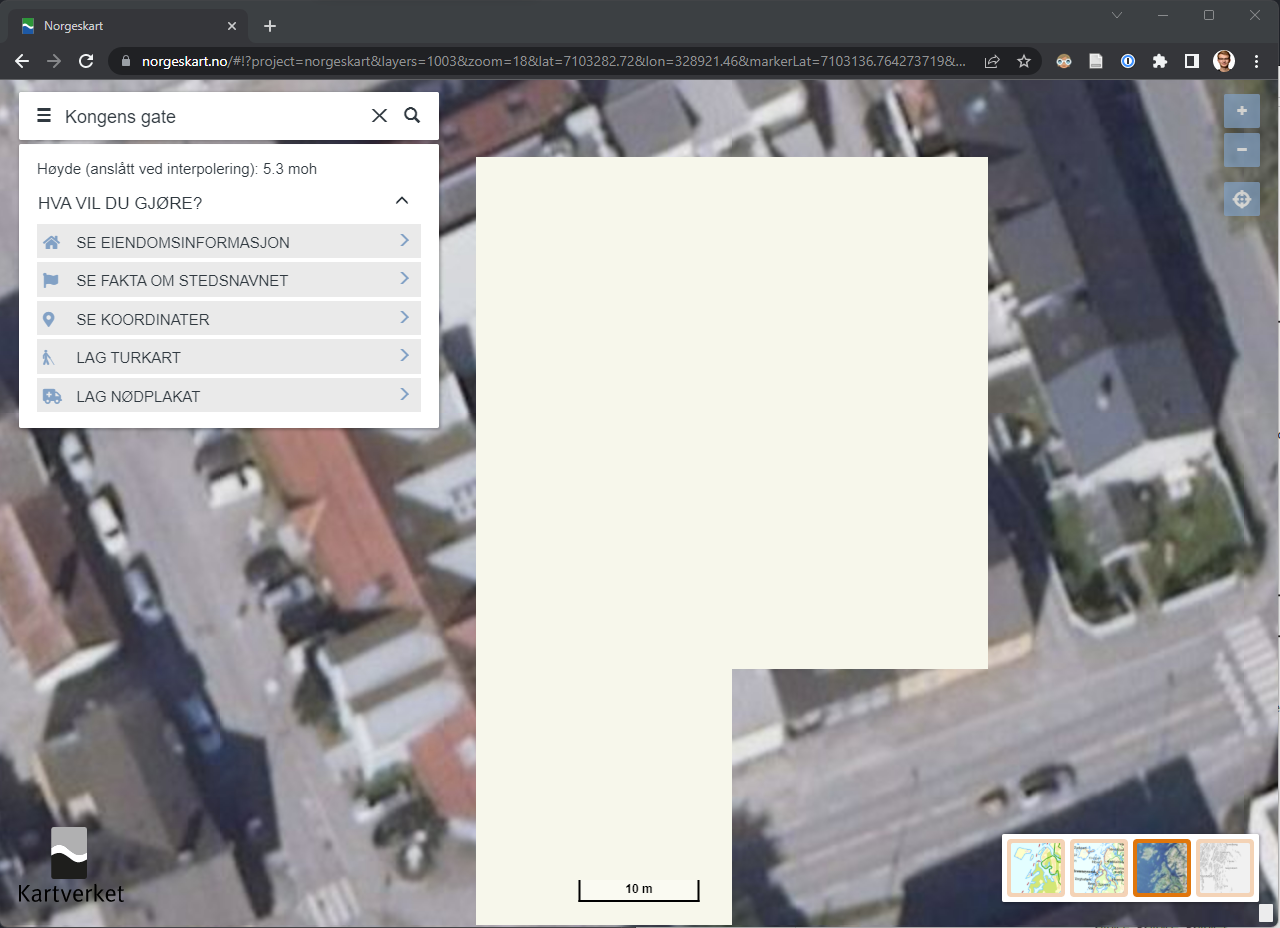
\includegraphics[width=.6\textwidth]{figures/gui/norgeskart_bug.png}
    \caption{Screenshot showing the white patches that appears when zoom level goes beyong \todo \cite{kartverketNorgeskart}}
    \label{fig:norgeskart_bug}
\end{figure}
\begin{figure}[H]
    \centering
    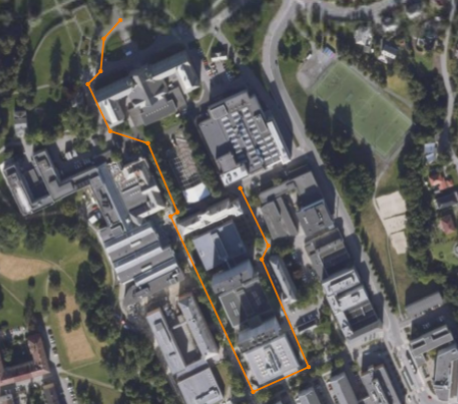
\includegraphics[width=.6\textwidth]{figures/gui/sattelite_with_plot.png}
    \caption{A plot showing how latitude and longitude data can be plottet on top of sattelite images}
    \label{fig:dash_sattelite}
\end{figure}